% 
% Annual Cognitive Science Conference
% Sample LaTeX Paper -- Proceedings Format
% 

% Original : Ashwin Ram (ashwin@cc.gatech.edu)       04/01/1994
% Modified : Johanna Moore (jmoore@cs.pitt.edu)      03/17/1995
% Modified : David Noelle (noelle@ucsd.edu)          03/15/1996
% Modified : Pat Langley (langley@cs.stanford.edu)   01/26/1997
% Latex2e corrections by Ramin Charles Nakisa        01/28/1997 
% Modified : Tina Eliassi-Rad (eliassi@cs.wisc.edu)  01/31/1998
% Modified : Trisha Yannuzzi (trisha@ircs.upenn.edu) 12/28/1999 (in process)
% Modified : Mary Ellen Foster (M.E.Foster@ed.ac.uk) 12/11/2000
% Modified : Ken Forbus                              01/23/2004
% Modified : Eli M. Silk (esilk@pitt.edu)            05/24/2005
% Modified: Niels Taatgen (taatgen@cmu.edu) 10/24/2006

%% Change ``a4paper'' in the following line to ``letterpaper'' if you are
%% producing a letter-format document.

\documentclass[10pt,letterpaper]{article}

\usepackage{cogsci}
\usepackage{bbm,amsmath,amssymb}
\usepackage{pslatex}
\usepackage{natbib}
\usepackage{bm}
\usepackage[usenames,dvipsnames]{xcolor}
\usepackage{tikz}
\usetikzlibrary{arrows}
\usepackage{verbatim}
\newcommand{\tb}[1]{\textcolor{Blue}{#1}}
%\usepackage{apacite}

\definecolor{Red}{RGB}{255,0,0}
\newcommand{\red}[1]{\textcolor{Red}{#1}}  

\title{A Resource-Rational Approach to the Causal Frame Problem}
 
 
\author{{\large \bf Thomas F. Icard, III} (icard@stanford.edu), {\large \bf Noah D. Goodman} (ngoodman@stanford.edu)\\
  Departments of Philosophy and Psychology, Stanford University}

\begin{document}

\maketitle


\begin{abstract}
The \emph{causal frame problem} is an epistemological puzzle about how the mind is able to disregard seemingly irrelevant causal knowledge, and focus on those factors that promise to be useful in making an inference or coming to a decision. Taking a subject's causal knowledge to be (implicitly) represented in terms of directed graphical models, the causal frame problem can be construed as the question of how to determine a reasonable ``submodel'' of one's ``full model'' of the world, so as to optimize the balance between accuracy in prediction on the one hand, and computational costs on the other. We propose a framework for addressing this problem, and provide several illustrative examples based on HMMs and Bayes nets. We also show that our framework can account for some of the recent empirical phenomena associated with alternative neglect.

\textbf{Keywords:} 
frame problem, bounded-resource-rationality, causal reasoning, alternative neglect.
\end{abstract}

\section{Introduction}

To any inference or decision problem, there is no \emph{a priori} bound on what aspects of a person's knowledge may be usefully, or even critically, applied. In principle, anything could be related to anything. 
This challenge is sometimes referred to as the \emph{frame problem}, characterized by \cite{Glymour1987} as: ``Given an enormous amount of stuff, and some task to be done using some of the stuff, what is the \emph{relevant stuff} for the task?'' (65). The question is foundational to reasoning and rationality. 
Part of what makes people so smart is our ability to solve the frame problem, ignoring those aspects of the world (and our knowledge of it) that are irrelevant to the problem at hand, thereby simplifying the underlying reasoning task, turning an intractable problem into a tractable one.

Not all of the psychological literature paints a picture of human reasoners as so adept at disregarding only the irrelevant, however. In the literature on causal reasoning, there is a robust empirical finding that subjects often neglect causal variables, including those that are in principle accessible to the subject, which would sometimes allow the subject to make better, more accurate inferences. So called \emph{alternative neglect} is an especially well documented phenomenon, in which subjects ignore alternative possible causes of some event (\citealt{Fischhoff1978,KlaymanHa,Fernbach2011}, \emph{inter alia}), even when doing so leads to incorrect inferences. More generally, at least in the causal domain, subjects seem to consider ``smaller'' models of the world than would be relevant to the task at hand, given the subject's knowledge and reasoning abilities. This has led many to criticize the behavior as normatively objectionable. Perhaps people are ignoring too much of their knowledge.

We would like to suggest that alternative neglect and related phenomena may be natural consequences of a general mechanism for sifting the most pertinent information from all other knowledge---that is, for solving the frame problem with regard to causal knowledge. Assuming a person's causal knowledge can be represented (at least implicitly) in terms of a very large directed graphical model (or Bayes net), the \emph{causal} frame problem arises because computations involving the entire model promise to be intractable. Somehow the mind must focus in on some ``submodel'' of the full model that suffices for the task at hand and is not too costly to use. In as far as a proper submodel may nonetheless neglect relevant causal information, this may lead to inaccuracy. We suggest that perhaps the mind tolerates local and occasional inaccuracy in order to achieve a more global efficiency. 
To substantiate this claim, we need a better understanding of what it is for a submodel to be more or less apt for a task, from the perspective of a reasoner with bounded time and resources. It is clear that human reasoners cannot consult an indefinitely detailed mental model of the world for every inference task. So what kind of simpler model \emph{should} a reasoner consult for a given task?

This work follows a line of research in cognitive science concerned with \emph{bounded} or \emph{resource rationality} (\citealt{Simon1957,Gigerenzer1996}, \emph{inter alia}), and specifically in the context of probabilistic models, and approximations thereto \citep{Vul2014}. In addition to inherent interest, it has recently been suggested that considerations of bounded rationality may play a methodological role in sharpening the search for reasonable accounts of the cognitive processes underlying inductive inference \citep{Griffiths2014,Icard2014}. However, in this tradition there has been more of a focus on the algorithm used for inference in a given model, and less attention paid to questions of model selection.

In this largely programmatic paper we offer a framework for addressing the causal frame problem by selecting rational submodels, provide several illustrative examples, and address some of the empirical findings concerning alternative neglect.

\section{Resource-Rational Submodels}

Let $P(\textbf{X})$ be a joint probability distribution over random variables $\textbf{X} = X_1,X_2,\dots$, and define a \emph{query} to be a partition $\langle \textbf{X}_q;\textbf{X}_l;\textbf{X}_e\rangle$ of \textbf{X} into \emph{query variables}, \emph{latent variables}, and \emph{evidence variables}, respectively. A typical query task is to find values of $\textbf{X}_q$ that maximize the conditional probability $P(\textbf{X}_q\mid \textbf{X}_e = \textbf{v})$, marginalizing over values of $\textbf{X}_l$. Clearly, the difficulty of this and related tasks scales with the number of variables. We will be interested in smaller models with fewer variables: a sublist $\textbf{X}^*$ of $\textbf{X}$ with associated distribution $P^*(\textbf{X}^*)$, and associated partition $\langle \textbf{X}_q;\textbf{X}_l^*;\textbf{X}_e^*\rangle$, so that only latent and evidence variables are ignored. In each of the cases considered here (HMMs and Noisy-Or Bayes nets), there will be a canonical way of choosing $P^*$ given $\textbf{X}^*$. 
%\red{NDG: hmm... treating as uniform doesn't really remove their effect. instead we want to treat them as fixed, or as independent and uniform each time they are the parent of another node. or maybe we treat them as independent of their parents, so its the parents we actually neglect? and maybe we should mention the specialness of noisy-or here??}

Given $P(\textbf{X})$ and $P^*(\textbf{X}^*)$, there are at least two kinds of questions we would like to ask. The first of these captures how well an agent will fare by using the approximate submodel, as compared with the full model, holding fixed a procedure for using this model to choose an action. For instance, the agent might use this distribution to compute expected utility, or to \emph{sample} from the model in order to approximate expected utility (see, e.g,. \citealt{Vul2014}). The second question asks how far off the approximate model is from the ``true'' model in its probabilistic predictions.\footnote{Strictly speaking, the second can be seen a special case of the first, with a logarithmic scoring rule \citep{Bernardo}.} \begin{enumerate}
  \item Given a decision problem with action space $\mathcal{A}$ and utility function $U:\textbf{X}_q\times \mathcal{A} \rightarrow\mathbb{R}$, and assuming fixed a (stochastic) choice rule $\Psi_Q$ taking a distribution $Q$ over $\textbf{X}_q$ to a distribution on actions, what are the respective expected utilities of using $P$ and $P^*$ under (assumed ``true'') distribution $P$? That is, how great is the following difference $\Delta_{P,P^*}$? \end{enumerate}
  $$\Delta_{P,P^*} \;\; = \;\; \mathbb{E}_{\textbf{x}\sim P}\;\mathbb{E}_{A \sim \Psi_{P}}\;U(\textbf{x},A) \,-\, \mathbb{E}_{\textbf{x} \sim P}\;\mathbb{E}_{A \sim \Psi_{P^*}}\;U(\textbf{x},A)$$
  \begin{enumerate}
  \item[2.] How far is $P^*$ from $P$ in information distance, for the variables $\textbf{X}_q$ of interest? That is, what is the Kullback-Leibler divergence between $P$ and $P^*$ with respect to $\textbf{X}_q$?
\end{enumerate}$$KL(P \;||\; P^*)  =  \sum_{\textbf{x}} P(\textbf{X}_q = \textbf{x} \mid \textbf{X}_{e} = \textbf{v})\; \mbox{log} \; \frac{P(\textbf{X}_q = \textbf{x} \mid \textbf{X}_{e} = \textbf{v})}{P^*(\textbf{X}_q = \textbf{x} \mid \textbf{X}^*_{e} = \textbf{v}^*)}$$
In general we will expect that $KL(P \;||\; P^*) > 0$, and $\mathbb{E}_{\textbf{x}\sim P}\;\mathbb{E}_{A \sim \Psi_{P}}\;U(\textbf{x},A) > \mathbb{E}_{\textbf{x} \sim P}\;\mathbb{E}_{A \sim \Psi_{P^*}}\;U(\textbf{x},A)$. However, in line with other work on resource rationality, assuming the requisite computations using distribution $P$ come with a greater cost than when using $P^*$, this difference in cost may well be worth the difference in accuracy or utility.

Suppose we have a cost function $c: \mathcal{P}\rightarrow\mathbb{R}^+$, assigning a real cost to each approximation $P^* \in \mathcal{P}$. For instance, $c$ may simply charge a constant amount for each variable used in the associated submodel, or may be proportional to a graph property such as tree width. Given a set $\mathcal{P}$ of approximations, we can then ask for the \emph{resource-optimal} approximation  in either of the above two senses. For instance, with KL-divergence, of interest is the distribution $\tilde{P}$ that optimally trades off cost against KL-distance from the true distribution $P$: 

\begin{equation} \tilde{P} \;\;= \;\; \underset{P^*\in\mathcal{P}}{\textnormal{argmin}} \; KL(P\;||\;P^*) + c(P^*)\;.\label{optimal}\end{equation}


In what follows we illustrate these ideas with three examples using familiar graphical models. The first example, of an HMM, demonstrates an extreme case of the frame problem in which the initial model is potentially infinite. In this case we show that the resource-optimal submodel is not only finite, but often quite small, and in many instances includes just a single node. The second example, of a causal Bayes net, shows that under a sampling scheme for decision making, the submodel actually outperforms the ``ideal'' full model in many cases, even without taking costs into account. Finally, the third example, also involving small Bayes nets, reveals that certain kinds of inferences may be subject to greater information loss resulting from resource-rational neglect than others. Recent empirical literature shows that people respect this difference, suggesting that there may indeed be an element of resource rationality in alternative neglect behavior.

\section{Hidden Markov Models}

A Hidden Markov Model is given by a time-labeled sequence of state variables $\dots,X_{-1},X_{0},X_1,\dots$, %\red{NDG: i think we need to number these the other way, to make them go back to infinity?} 
with transition probability $P(X_{t+1}\mid X_t)$, and a sequence of evidence variables $\dots,Y_{-1},Y_0,Y_1,\dots$, with emission probabilities $P(Y_t\mid X_t)$. In a typical inference task, after observing  values of $Y$ (blue), we are interested in the value of $X_{t+1}$ (beige) at time $t+1$:

\begin{figure}[h] 
\begin{center}
  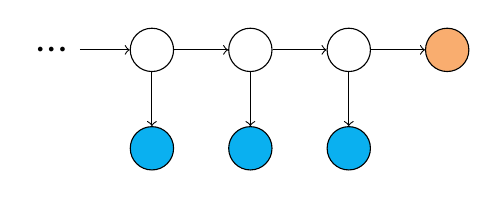
\begin{tikzpicture}
  
  
  \node (s0) at (-.25,1.25)  {$\textbf{\dots}$};
  
  \node (s1) at (1,1.25) [circle,draw=black,minimum size=0.55cm] {};

  \node (s2) at (1,0) [circle,draw=black,fill=ProcessBlue,minimum size=0.55cm] {};
  
  \node (s3) at (2.25,1.25) [circle,draw=black,minimum size=0.55cm] {};
  
  \node (s4) at (2.25,0)  [circle,draw=black,fill=ProcessBlue,minimum size=0.55cm] {};
  
  \node (s5) at (3.5,1.25) [circle,draw=black,minimum size=0.55cm] {};
  
  \node (s6) at (3.5,0)  [circle,draw=black,fill=ProcessBlue,minimum size=0.55cm] {};
  
  \node (s7) at (4.75,1.25) [circle,draw=black,minimum size=0.55cm,fill=Apricot] {};
 
  \path (s0) edge[->] (s1);
  
  \path (s1) edge[->] (s2);
  
  \path (s1) edge[->] (s3);
  
  \path (s3) edge[->] (s4);
  
  \path (s3) edge[->] (s5);
  
  \path (s5) edge[->] (s6);
  
  \path (s5) edge[->] (s7);
  
 \end{tikzpicture}
\end{center} 
\end{figure} 
\noindent For instance, variables $X$ might be whether there is high or low air pressure, while observations $Y$ are of sun or clouds. While in principle determining $X_{0}$---what the weather will be like today---could depend on indefinitely earlier observations and states at times $t=-1,-2,\dots$---indeed, the model could even be infinite---one has the intuition that ``looking back'' only a few steps should be sufficient for typical purposes.

For a first illustration, consider a simple HMM with binary variables $X_t$ and $Y_t$, and probabilities as follows:
$$P(X_{t+1}=1\mid X_t=1) = P(X_{t+1}=0\mid X_t=0) = 0.9$$
$$P(Y_{t}=1\mid X_t=1) = P(Y_{t}=0\mid X_t=0) = 0.8$$
Our class $\mathcal{P}$ of approximate distributions includes all truncations of the model at variable $X_{t-N}$, in which case we assume the distribution $P^{*}(X_{t-N})$ is uniform. In Figure \ref{hmm}1 is a graph showing the KL-distance between the full model and a submodel with only $N$ previous time steps included.
 \begin{figure}[h]  \begin{center}
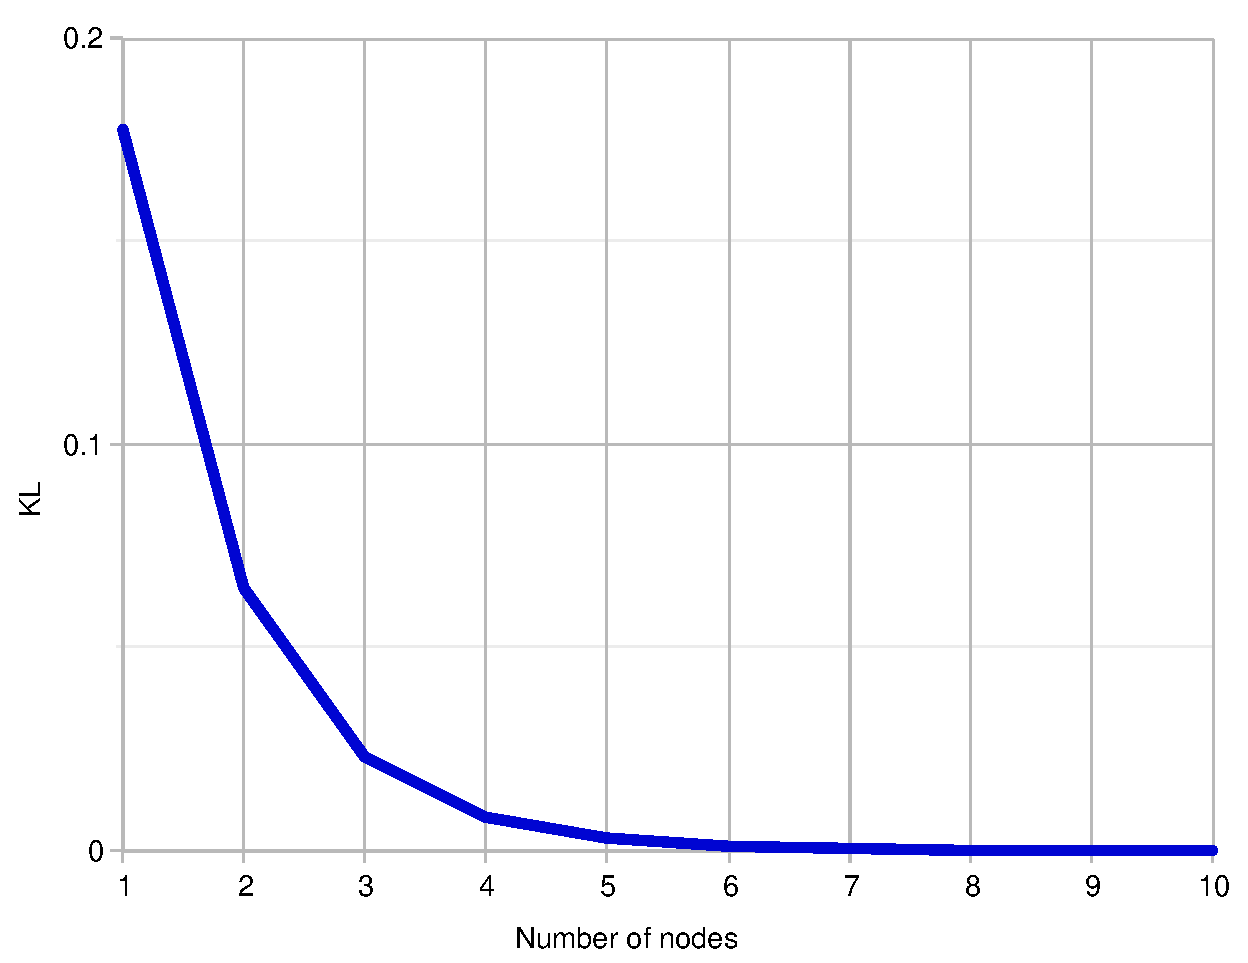
\includegraphics[scale=0.3]{hmm1.pdf} \caption{Dropoff in KL as function of number of nodes.} \end{center} 
\label{hmm}\end{figure} 
We chose this particular model for illustration because the KL-distance is relatively high for the submodel with only one node. Nonetheless, even for this model, the value drops off rather dramatically with only a few additional nodes. This model has a low mixing rate, as measured by the second eigenvalue ($\lambda_2$) of the transition matrix for the underlying Markov model (the transition probabilities). In general, a higher $\lambda_2$ value means a lower mixing rate. One might expect that in such cases it is more detrimental to ignore previous state variables. If we look at the graph (Figure \ref{kl-eigen}2) of KL-distances as a function of $\lambda_2$, holding fixed the observation probabilities as above, we see that this model (for which $\lambda_2 = 0.8$) is indeed near the higher end.

 \begin{figure}[h]  \begin{center}
 \label{kl-eigen}
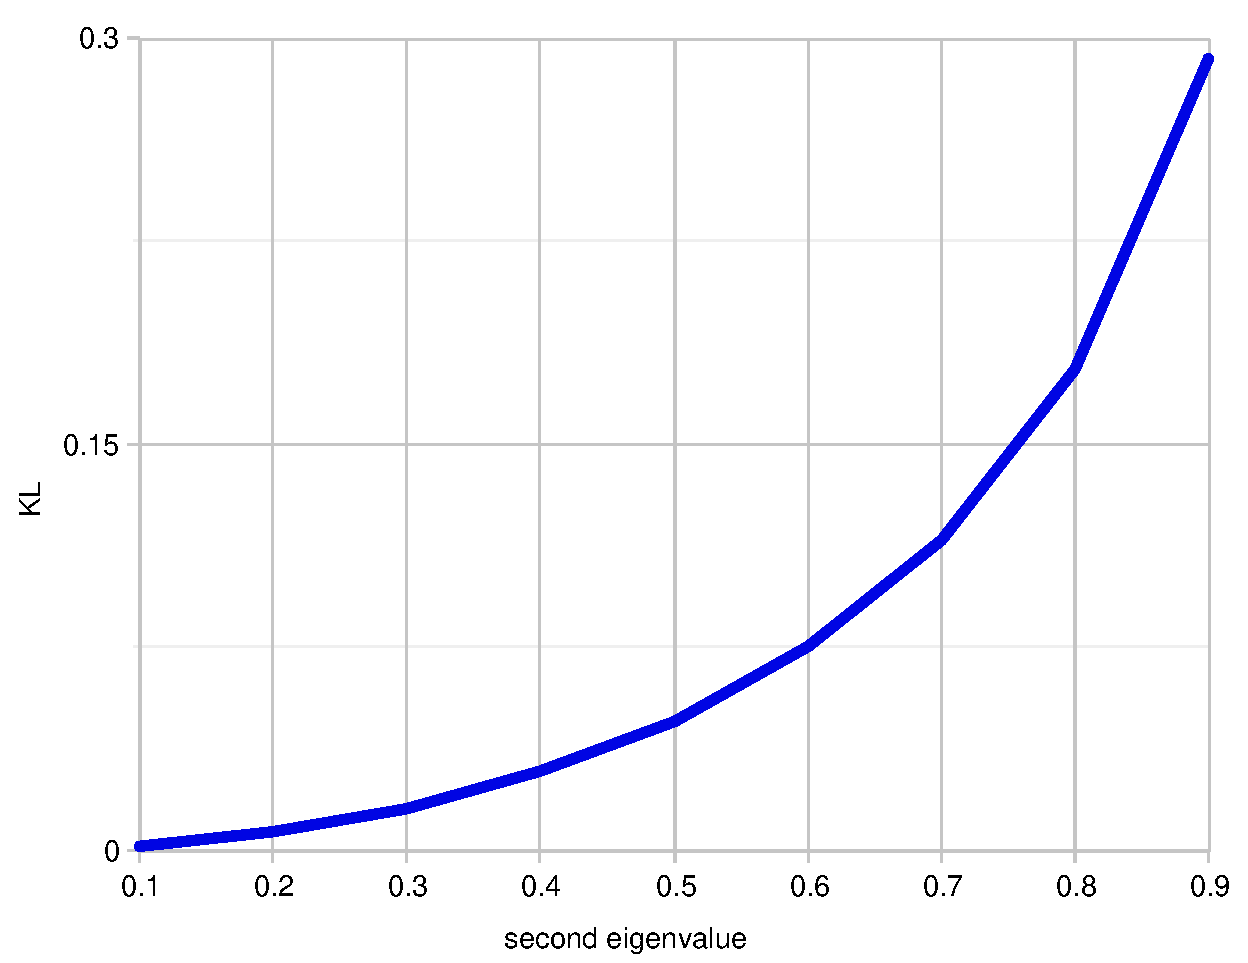
\includegraphics[scale=0.33]{kl-eigenvalue-5.pdf} \caption{KL-distance for an approximate model with only one state variable, as a function of second eigenvalue $\lambda_2$.} \end{center} 
\end{figure}

If we now factor in the cost of including more nodes in the approximate HMM, we can determine for different values of $\lambda_2$, and for different assumptions about cost of a node, what the optimal number of nodes to include will be, in line with the Equation (\ref{optimal}) above. To give one (arbitrary, but illustrative) example, in the following graph we assume the cost of an additional node to be $0.02$, i.e., that this cost is equivalent to $\frac{1}{50}$ of a bit of information.%\footnote{Recall that KL measures the average number of additional bits required to code samples from $P*$ with an optimal code for $P$.}

 \begin{figure}[h]  \begin{center}
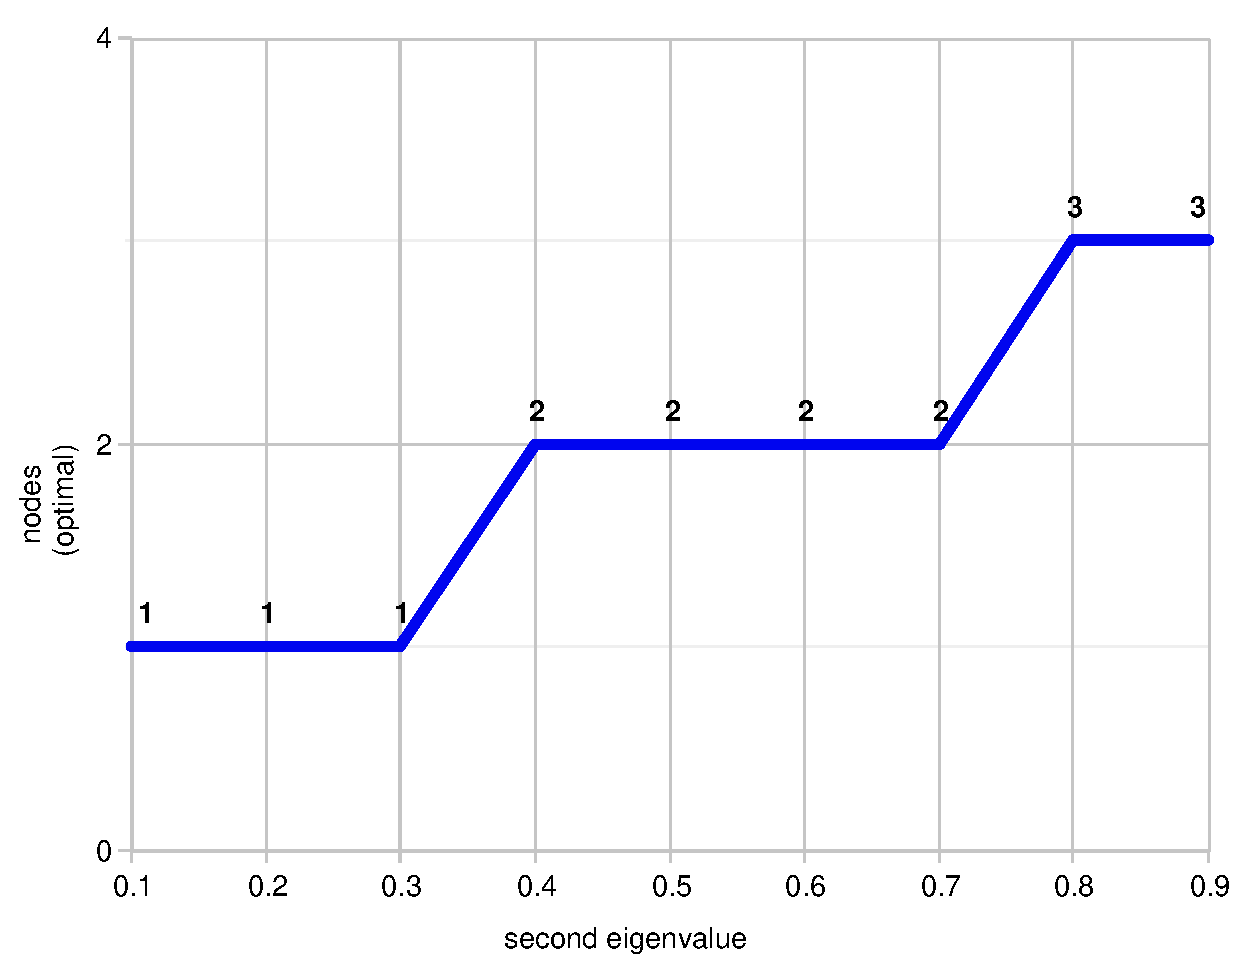
\includegraphics[scale=0.33]{kl-eigenvalue-7.pdf} \caption{Optimal number of nodes, given a cost of $0.02$ per node, as a function of second eigenvalue $\lambda_2$.} \end{center} 
\label{kl-eigen1}\end{figure}

\noindent For relatively low values of $\lambda_2$, it is not worth the cost to include more than a single state variable in the model. This is perhaps not surprising, given the low KL-values in Fig. \ref{kl-eigen}2. However, even in models with significantly higher KL-distances in general, it does not pay to include more than one or two additional nodes. %Note in particular that, while a model with $\lambda_2=0.8$ is further from the true model than one with $\lambda_2=0.7$, only in the latter case does the marginal difference in KL-value between including two and three nodes merit the cost of including the third node. 
%\red{is it weird that is wiggles at the end?}
%TFI: It does seem to wiggle for various parameter settings, but I changed the parameters (so that observation probs are 0.8, not 0.9), which gave a nicer(?) graph.
As we increase or decrease the cost $c$ of a node, this graph becomes less flat and flatter, respectively. For instance, as long as $c>0.148$, the optimal number is 1 for all these values of $\lambda_2$. Decreasing the cost would increase the optimal number for larger values of $\lambda_2$, but for any $c>0$ this number is of course still finite.

As Fig. \ref{kl-eigen1}3 indicates, the optimal number of nodes to include in an HMM is not only finite, but can typically be quite small.

\section{Neglecting Alternative Causes}

We next consider a simple causal model under a so called Noisy-Or parameterization \citep{Cheng}. Suppose we have binary causal variables $\textbf{X}$, taking on values 0 or 1, and conditional probabilities given in terms of weights $\theta_{Y,X}$ codifying the influence of parent $Y$ on a variable $X$---in particular $\theta_{Y,X}$ gives the probability of $Y$ causing $X$ when $Y$ is active ---and a ``background bias'' parameter $\beta$: $$P\big(X\mid \textbf{pa}(X)\big) \quad = \quad 1-\Big((1-\beta)\prod_{Y \in \textbf{pa}(X)} (1-\theta_{Y,X})^Y\Big)$$
This model has the convenient property that, deleting nodes from the graph still leaves us with a well-defined distribution. Hence the family of sub-models is immediate from the full model (without having to introduce proxy uniform distributions as in previous example).

Suppose in particular we have variables $A,B,C,D$ with weights $\theta_1, \theta_2$, and $\theta_3$, as depicted on the left in Figure \ref{noisy-or}.
\begin{figure}[h] 
\begin{center}
  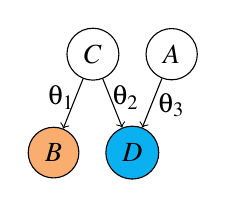
\begin{tikzpicture}
  
  \node (s0) at (.5,1.25) [circle,draw=black] {$C$};
  
  \node (s1) at (1.5,1.25) [circle,draw=black] {$A$};
  
  \node (s2) at (0,0) [circle,draw=black,fill=Apricot] {$B$};
  
  \node (s3) at (1,0) [circle,draw=black,fill=ProcessBlue] {$D$};
 
  \path (s0) edge[->] (s2);
  
  \path (s0) edge[->] (s3);
  
  \path (s1) edge[->] (s3);
  
  \node (i1) at (.1,.7) {$\theta_1$};
  
  \node (i1) at (.92,.7) {$\theta_2$};
  
  \node (i1) at (1.5,.6) {$\theta_3$};
  
 \end{tikzpicture} \hspace{0.7in}
   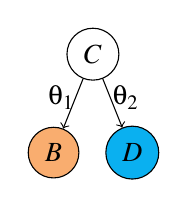
\begin{tikzpicture}
  
  \node (s0) at (.5,1.25) [circle,draw=black] {$C$};
  
  \node (s2) at (0,0) [circle,draw=black,fill=Apricot] {$B$};
  
  \node (s3) at (1,0) [circle,draw=black,fill=ProcessBlue] {$D$};
 
  \path (s0) edge[->] (s2);
  
  \path (s0) edge[->] (s3);
  
  \node (i1) at (.1,.7) {$\theta_1$};
  
  \node (i1) at (.92,.7) {$\theta_2$};
  
 \end{tikzpicture}
\end{center} \caption{Full Model versus Partial Submodel} \label{noisy-or}
\end{figure} 

\noindent Imagine, for instance, a case of social reasoning, in which: \begin{itemize} \item[] $A$: ``Mary has lost her usual gloves'' \item[] $B$: ``Mary has her bicycle with her''  \item[] $C$: ``Mary is going cycling"  \item[] $D$:  ``Mary is wearing cycling gloves'' \end{itemize}
Observing that Mary is wearing cycling gloves makes it more likely that she is going cycling, and therefore that she has her bike with her. But this is attenuated by the alternative possible cause, that she lost her other gloves. Our question in this case is, how much worse will a reasoner fare by ignoring alternative cause $A$, that is, by using the smaller submodel  in Figure \ref{noisy-or}, on the right?

To assess this question, we can look at both the difference in expected utility and the KL-divergence between using the ``true'' distribution $P$ and the approximate distribution $P^*$, for $B$ given $D=1$. Table \ref{table1} below presents example KL-values for different settings of model parameters (here and throughout this subsection, we set $\beta = 0.05$).

\begin{table}[h]  \begin{center}
\begin{tabular}{c | c | c | c | c || c}
 $P(C)$ & $P(A)$ & $\theta_1$ & $\theta_2$ & $\theta_3$ & $KL(P \;\vert\vert\; P^*)$ \\ \hline
 $0.5$ & $0.5$ & $1$ & $1$ & $1$  & $0.594$ \\
  $0.5$ & $0.5$ & $1$ & $0.5$ & $0.9$  & $0.467$ \\
  $0.5$ & $0.5$ &$1$ & $0.5$ & $0.5$  & $0.270$ \\
 $0.5$ & $0.5$ & $1$ & $0.9$ & $0.5$  & $0.261$ \\
  $0.3$ & $0.1$ & $1$ & $1$ & $1$ & $0.121$ \\
 $0.5$ & $0.5$ &  $0.9$ & $0.1$ & $0.5$  & $0.081$ \\
  $0.3$ & $0.1$ & $0.9$ & $0.1$ & $0.5$ & $0.023$ \\
 $0.5$ & $0.5$ & $0.1$ & $0.1$ & $0.1$ & $0.000$ 
\end{tabular} \end{center} \caption{Example KL-values, with $\beta = 0.05$.} \label{table1}
\end{table}
Table \ref{table1} in fact shows settings near the higher end. We can also calculate the approximate \emph{average} KL-divergence, over values of $P(C)$ and $P(A)$ at $0.1$ intervals ($0.1$, $0.2$, etc.), and $0.01$ intervals for $\theta_1,\theta_2,\theta_3$ (thus, over 7 million parameter settings): for this model, it is $0.060$. Averaging over parameters with $P(A)$ and $P(C)$ fixed at $0.5$ gives a similar value of $0.059$.
Thus, the KL-value is typically much lower than the higher values in Table \ref{table1}. Nonetheless, if confidence in estimation is important, or if more fine-grained decisions are called for, using a submodel in this case may be detrimental. 

However, following question 1 from above, we may also consider how detrimental using a submodel will be for action choice in specific decision problems.
For the EU calculation, suppose our agent is making a guess based on a single sample from distributions $P$ and $P^*$,\footnote{This assumption is more apt in more complicated models, where computing exact estimates would be harder. We consider this kind of rule simply for illustration, and contrast with information distance, which would be more closely aligned with an agent (non-noisily) maximizing expected utility across decision problems.\label{fn}} and that utility 1 is achieved for a correct response, 0 for incorrect. Example calculations are summarized in Table \ref{table2}.

\begin{table}[h]  \begin{center}
\begin{tabular}{c | c | c | c | c || c}
 $P(C)$ & $P(A)$ & $\theta_1$ & $\theta_2$ & $\theta_3$ & $\Delta_{P,P*}$ \\ \hline
 $0.5$ & $0.5$ & $1$ & $1$ & $1$  & $-0.097$ \\
  $0.5$ & $0.5$ & $1$ & $0.5$ & $0.9$  & $-0.074$ \\
  $0.5$ & $0.5$ &$1$ & $0.5$ & $0.5$  & $-0.087$ \\
 $0.5$ & $0.5$ & $1$ & $0.9$ & $0.5$  & $-0.096$ \\
  $0.3$ & $0.1$ & $1$ & $1$ & $1$ & $-0.073$ \\
 $0.5$ & $0.5$ &  $0.9$ & $0.1$ & $0.5$  & $-0.007$ \\
  $0.3$ & $0.1$ & $0.9$ & $0.1$ & $0.5$ & $0.011$ \\
 $0.5$ & $0.5$ & $0.1$ & $0.1$ & $0.1$ & $0.006$ 
\end{tabular} \end{center} \caption{Example EU-values, with $\beta = 0.05$.} \label{table2}
\end{table}
%NDG: we should introduce the idea of using a submodel with an approximate inference algorithm earlier. we can there point out that the best submodel may be different depending on the (approximate) inference algorithm used, and set up the one-sample case. here we should first do the full conditional version, then the one-sample version.
%TFI: Okay, I added a bit above. Should we say even more?

 \noindent As with KL, we can also compute the (approximate) average difference in EU, which for this model is $0.024$. That is, on average over all parameter settings, a sampling agent will only suffer about $\frac{1}{50}$ of a utile by using the simpler submodel.

Evidently, when making a binary, sample-based decision, using the smaller submodel does not greatly reduce one's success probability. In fact, as shown in Table \ref{table1}, for many parameter settings the agent actually fares better by using the simpler model. Take the first parameter setting, for example. In this case $P(B=1\mid D=1) \approx 0.673$, whereas $P^*(B=1 \mid D=1) \approx 0.955$. The submodel drastically overestimates the probability of $B$ by ignoring the alternative cause, as reflected in the very high KL-value. However, insofar as the true probability is significantly above $0.5$, if the subject is going to make a decision by drawing a single sample from this distribution, such overestimation turns out to be advantageous, since the subject is more likely to choose the more probable outcome. Such advantages would only be compounded by the reduction in computational cost resulting from the simpler model.

We can tentatively conclude from this small case-study that alternative neglect---even when it results in less accurate judgments, which it certainly does---can be resource-rational. 

\section{Predictive versus Diagnostic Reasoning}

Resource-rational analysis of submodel choice and alternative neglect predicts these phenomena to occur, at least to a first approximation, when they would result in resource-rational choice and action, as outlined above. To what degree is this prediction born out by the data on alternative neglect?

One of the more robust recent findings in the causal reasoning literature is that subjects tend to neglect alternatives to a much greater extent in \emph{predictive} reasoning than in \emph{diagnostic} reasoning \citep{Fernbach2011,Fernbach2013}. Most of the experiments in this work evince three variables $A,B,C$ as in Figure \ref{diagnostic}.
\begin{figure}[h] \begin{center}
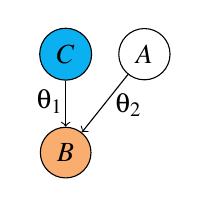
\begin{tikzpicture}
  \node (s0) at (0,1.25) [circle,draw=black,fill=ProcessBlue] {$C$};
  
  \node (s2) at (0,0) [circle,draw=black,fill=Apricot] {$B$};
  
  \node (s3) at (1,1.25) [circle,draw=black] {$A$};
 
  \path (s0) edge[->] (s2);
  
  \path (s3) edge[->] (s2);
  
  \node (l1) at (-.2,.65) {$\theta_1$};
  
  \node (l1) at (.8,.6) {$\theta_2$};
  
 \end{tikzpicture}
\hspace{.7in}
  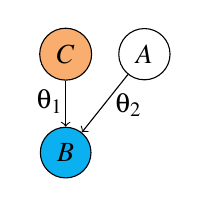
\begin{tikzpicture}
  
  \node (s0) at (0,1.25) [circle,draw=black,fill=Apricot] {$C$};
  
  \node (s2) at (0,0) [circle,draw=black,fill=ProcessBlue] {$B$};
  
  \node (s3) at (1,1.25) [circle,draw=black] {$A$};
 
  \path (s0) edge[->] (s2);
  
  \path (s3) edge[->] (s2);
  
    \node (l1) at (-.2,.65) {$\theta_1$};
  
  \node (l1) at (.8,.6) {$\theta_2$};
  
 \end{tikzpicture} \end{center}
 \caption{Predictive versus Diagnostic Inference} \label{diagnostic}
\end{figure}
The left diagram depicts a predictive inference, where effect $B$ is queried given evidence that cause $C$ is active. On the right is a diagnostic inference, where the causal variable $C$ is queried given evidence $B$. In this simple model, we can fold $P(A)$ and $\theta_{B,A}$ into a single parameter $\theta_2$, so that $A$ effectively has prior probability 1, and the resulting conditional probabilities can be simplified to: 
$$P(B\mid C) \;= \; \theta_1 + \theta_2 - \theta_1\theta_2$$
$$P(C \mid B) \;= \; 1- \big(1-P(C)\big)\Big(\theta_2\;/\;\big(P(C)\theta_1 + \theta_2  - P(C)\big)\Big)$$
The finding in \cite{Fernbach2011} is that subjects routinely ignore variable $A$ in predictive inference tasks, and thereby consistently make low estimates of $P(B\mid C)$. In diagnostic inference tasks, however, subjects show sensitivity to strength and number of alternatives, consequently making more accurate judgments. Indeed, there is a longer reaction time for diagnostic than for predictive inferences, and only in the diagnostic condition is there dependency of reaction time on number of alternatives \citep{Fernbach2010}. \cite{Fernbach2013} verified that this asymmetry between diagnostic and predictive reasoning is robust; in particular, it seems not to be due to availability or memory limitations.

In other words, subjects seem to be reasoning with a submodel (ignoring variable $A$) in the predictive case, but not in the diagnostic case. How detrimental would it be to neglect $A$ for these two types of inference? Consider first KL-divergence (question 2). Without a background bias term (as in the previous example), for the diagnostic case ignoring variable $A$ will lead to the conclusion that $C$ has probability 1, since it is the only possible cause. In that case, the KL-divergence is not even defined. With a positive bias term $\beta$, we can make the KL-divergence as large as we like, by making the bias smaller. For instance, with $\beta = 0.01$, the average value of $KL(P\;||\;P^*)$ for the diagnostic inference is already $1.740$, extremely high. With $\beta=0.05$, it is $0.916$.

By contrast, the average value of $KL(P\;||\;P^*)$ in the predictive case (even without a bias term, which would further decrease the average KL value) is only $0.357$, significantly lower.  This is a general observation about this particular causal graph, which is the one implicated in the studies discussed. While it may be difficult to assess these KL-values absolutely, we can confirm that there is a substantial difference between the two types of inference. Indeed, on average one can expect to make much worse predictions in the diagnostic case than in the predictive case.

How does this look from the perspective of expected utility, again assuming a single-sample-based agent?  Table \ref{predictive} shows the differences in expected utility for several parameter settings between the EU of using the true distribution and the approximate distribution (ignoring variable $A$), for both the predictive and diagnostic cases. 
\begin{table}[h]  \begin{center}
\begin{tabular}{c | c | c || c | c}
 $P(C)$ & $\theta_1$ & $\theta_2$ & $\Delta_{pred}$ & $\Delta_{diag}$ \\ \hline
  $0.1$ & $0.3$ & $0.9$ & $1.083$ & $1.345$ \\
 $0.5$ & $0.9$ &  $0.9$ & $0.176$ & $-0.041$ \\
 $0.5$ & $0.5$ & $0.1$ & $0.010$ & $-0.144$ \\
  $0.2$ & $0.3$ & $0.2$ & $-0.034$ & $0.345$ \\
 $0.1$ & $0.3$ & $0.1$ & $-0.036$ & $0.550$ \\

\end{tabular} \end{center} \caption{Differences in expected utility between the true and approximate distributions, for predictive and diagnostic inferences (with $\beta = 0.05$ for diagnostic cases).} \label{predictive}
\end{table} 
In some cases, $\Delta_{pred}$ is indeed smaller than $\Delta_{diag}$, meaning that the agent suffers less in expected utility when using the smaller submodel. However, there are also cases where $\Delta_{pred}$ is greater than $\Delta_{diag}$. Indeed, the average $\Delta_{pred}$ value, over $0.01$ intervals for all parameters, is $0.198$---relatively large, and significantly greater than $\Delta_{diag}$, whose average is $0.044$. Again, this means that a subject drawing a single sample will on average lose about $\frac{1}{5}$ of a utile for predictive inferences on this graph, versus only about $\frac{1}{25}$ for diagnostic inferences.

If we take resource rationality as a working methodological hypothesis, we might conclude that for this particular graphical model, subjects are not typically making decisions based on a single sample. To be sure, the models in Fig. \ref{diagnostic} are rather simple, and one might expect that, once such a model (or submodel thereof) is considered, a subject will have little difficulty maximizing simple expectations (e.g., of utility) over this distribution, by drawing further samples, or by some other algorithmic method (cf. Fn. \ref{fn}). We have already seen that the average KL-distance is greater in the case of diagnostic inferences, but what if we compare action selection directly, for agents that accurately maximize expected utility?

It turns out that, for such agents, the average difference in EU over all parameter settings is indeed significantly greater in the diagnostic case ($0.378$, versus $0.174$ in the predictive case), suggesting again that, if one were to ignore causal variables in one case but not the other, it would seem to be most rational to do so in the predictive case, as subjects in fact do. 

We might therefore tentatively conclude that, at a certain level of grain, subjects are ignoring variables in a reasonable way. However, this does not yet say anything about resource-rationality at the level of individual inferences. In fact, \cite{Fernbach2013} have shown that subjects exhibit neglect even in cases where the mistake is rather serious, resulting in egregiously wrong predictions. One possible explanation is that subjects are optimizing grain of representation only at a high level of abstraction, in terms of general features of the inference problem (e.g., whether it is predictive or diagnostic). This hypothesis merits further empirical investigation, as well as further theoretical consideration, for instance, by incorporating elements of metalevel control \citep{Icard2014,Lieder2014} into the framework. The analysis offered here, we believe, promises a useful starting point for understanding how rational submodels might be selected online, and for addressing this question of level of grain.

\section{Further Questions and Directions}

The notion of \emph{rational submodel} presented here is from a ``god's eye'' point of view, determining which submodel of a larger model an agent ought to use for a given purpose, balancing costs with accuracy. As we have seen, the framework does already shed light on a number of phenomena: it agrees with our pretheoretical intuition that only a few previous time steps should matter in an HMM; it interacts in subtle ways with different assumptions about choice rules, witness the single-sampling agent in the second example; and it retrodicts general patterns observed in human causal reasoning data.

As an approach to the causal frame problem, the claim is that, somehow or other, the mind is able to focus attention on reasonable submodels for the task at hand. Of course, this leaves open a number of questions. Most saliently, how is the mind able to do this online, at inference time?

There is some empirical work on specific questions of this sort, e.g., when subjects will ``add'' a new causal variable in the face of further evidence (see, e.g., the \emph{contradiction hypothesis} of \citealt{Park}). Continuing with the idea of bounded-resource-rational analysis, we might try to understand the (resource-)rational basis of different algorithms for selecting a causal model with which to reason. As with other instances of rational analysis, this could then be used to focus attention on promising hypotheses for how the mind actually achieves this higher-order task. The framework in this paper is an important start on this question, insofar as the target of any such mechanism will be to identify submodels that are rational in exactly our ``god's eye'' sense.

There are also further ways we might compare causal models with respect to resource-efficiency. We studied mainly optimal number of nodes, from the perspective of KL-divergence, average utility for a sampling agent, and in the last case average utility for an expected utility maximizer. One could also consider other types of submodels, not by eliminating nodes, but, e.g., by cutting links.

Another natural question to consider is what the optimal \emph{combination} of submodel together with number of samples will be for a given model (thus combining the analysis here with that in \citealt{Vul2014}). Assuming smaller submodels will allow for more samples per unit of time (or energy), and given that more samples lead to more accurate predictions with respect to that model, there is a substantive question of what combination is optimal in any case.

One might also consider the same questions with respect to an agent using some specific algorithmic inference strategy, such as Markov Chain Monte Carlo or belief propagation (see \citealt{Griffiths2014} for discussion of MCMC is resource-rational psychological model, and \citealt{WickMcCallum} for work in AI of a similar spirit on ``query-aware'' MCMC). That is, given an agent that is using a specific inference strategy, what would be the optimal submodel for that strategy. This too can be combined into one optimization question: which model and what use of this strategy (e.g., how long of a burn-in) together give the best results?

To repeat, the precise level of grain at which the mind does efficiently solve this problem remains an open question. But we hope to have made some progress toward an answer to this question. We believe the question is central to  human reasoning. As Fodor remarked, ``The frame problem goes very deep; it goes as deep as the analysis of rationality" \citeyearpar{Fodor1987}.

%NDG: should do joint optimization of samples and submodel.
%TFI: Yes!

\subsection{Acknowledgements} Thanks to Andreas Stuhlm\"{u}ller and Long Ouyang for comments on a draft of this paper.

\bibliographystyle{apalike}

\bibliography{bayes}


\end{document}
